\chapter{電路系統}

\section{接線圖}

\begin{figure}[hbt!]
\begin{center}
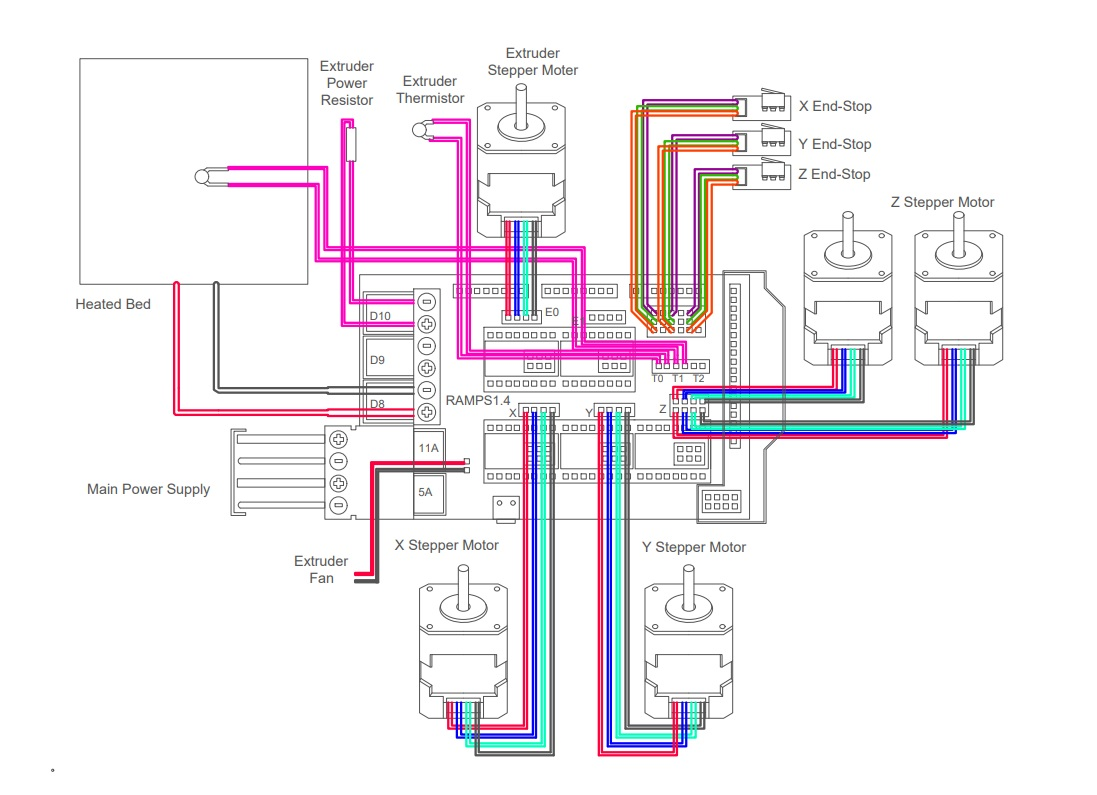
\includegraphics[width=18cm]{接線圖}
\caption{\Large 接線圖}\label{接線圖}
\end{center}
\end{figure}

\section{Arduino Mega 2560}
 Arduino Mega 2560 是基於ATmega2560的主控開發板。Arduino Mega 2560是採用USB接口的核心電路板。它具有54個數位輸入輸出,適合需要大量複雜I/O接口的設計。核心處理器為ATmega2560,有內建Pull-Up電阻在IC內部,不需要在外部電路另外安排Pull-Up電阻,同時具有54路數位輸入/輸出口、16個類比輸入,4個UART接口、1個16MHz晶體振盪器、1個USB連接口、1個電源插孔、1個ICSP接頭以及1個復位按鈕。Arduino Mega 2560也能兼容爲Arduino NUO設計的擴展板。可以自動選擇3中供電方式:外部直流電源通過電源插座供電;電池連接電源連接器的GND和VIN引腳;USB接口直流供電,整合了微控制器以及燒錄功能於一身。\\

\begin{figure}[hbt!]
\begin{center}
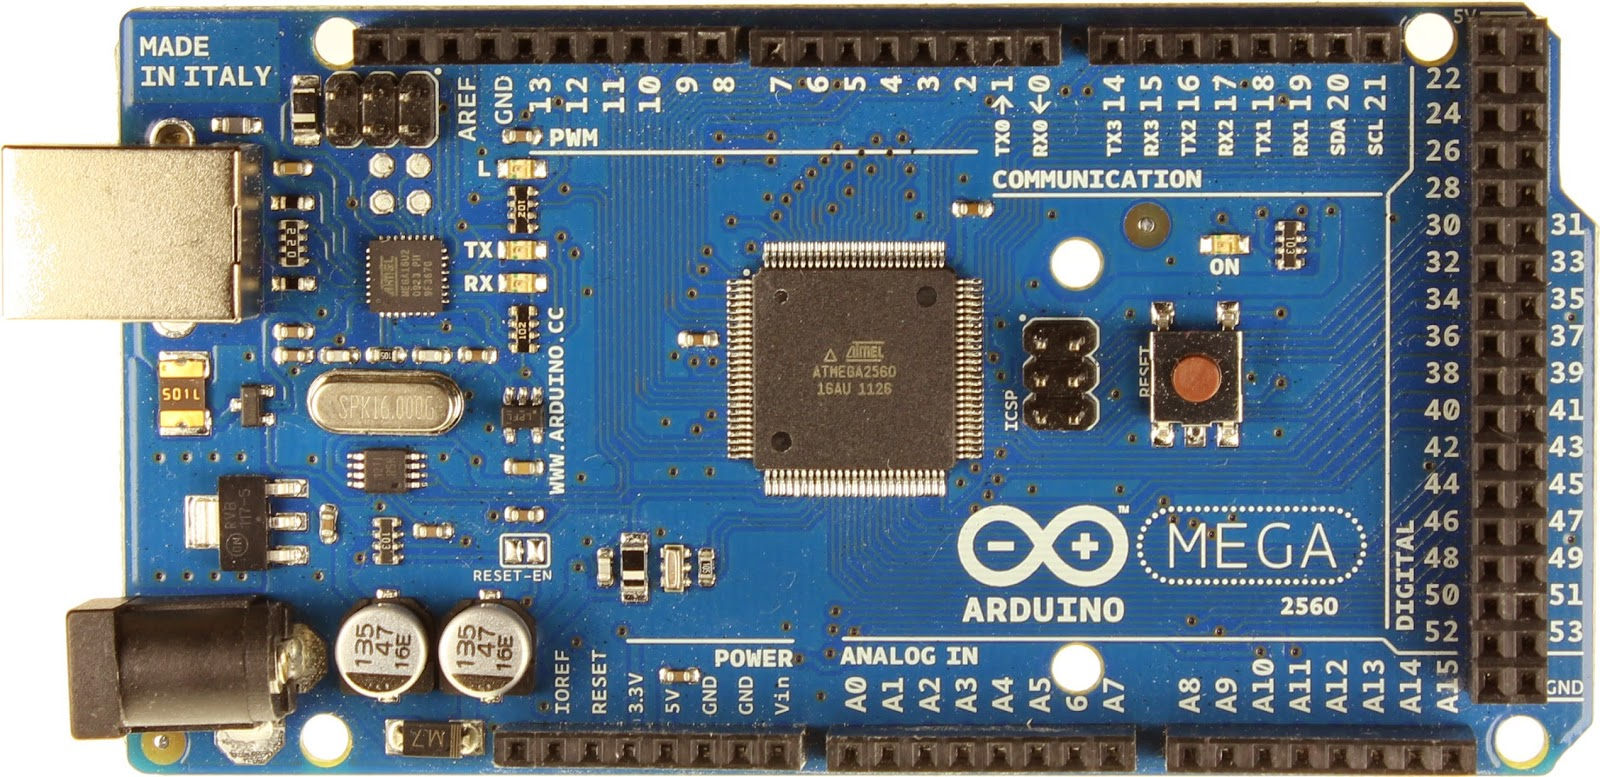
\includegraphics[width=16cm]{ArduinoMega2560}
\caption{\Large Arduino Mega 2560}\label{ArduinoMega2560}
\end{center}
\end{figure}

\newpage

\section{RAMPS 1.4}
 RAMPS 1.4 為RepRap Arduino Mega Pololu Shield的縮寫,主要為設計給步進馬達驅動器的介面電路,1.4為電路版本號碼,目前最新版本為1.7,Arduino Mega 2560可透過RAMPS 1.4介面與控制電路溝通進而達成控制步進馬達以及其他硬體的功能,目前可控制X、Y、Z三軸與最多兩個擠出頭以及兩個散熱風扇。\\
\begin{figure}[hbt!]
\begin{center}
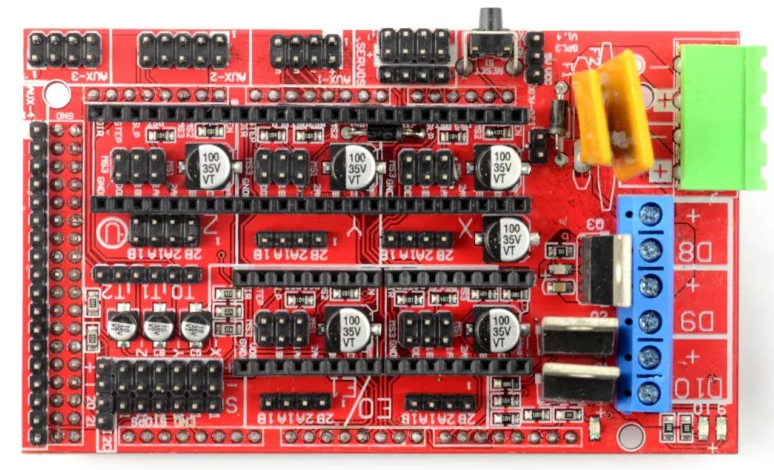
\includegraphics[width=14cm]{Ramps}
\caption{\Large RAMPS 1.4}\label{Ramps}
\end{center}
\end{figure}

\section{其餘元件}
 
\begin{figure}[hbt!]
\begin{center}
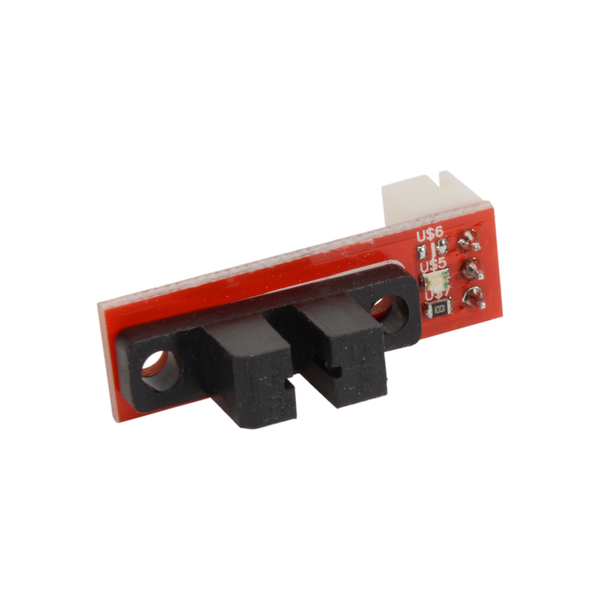
\includegraphics[width=8cm]{endstop}
\caption{\Large 光學限位開關(optical endstop switch)}\label{endstop}
\end{center}
\end{figure}

 光學限位開關的連接需要用到3條線,分別接到RAMPS上的(S)、(-)及(+),這3個腳位。\\

\newpage

\begin{figure}[hbt!]
\begin{center}
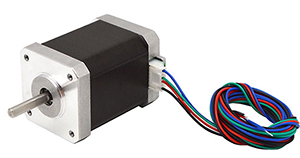
\includegraphics[width=8cm]{NEMA17}
\caption{\Large 步進馬達(Nema 17 Stepper Motors)}\label{NEMA17}
\end{center}
\end{figure}
\begin{figure}[hbt!]
\begin{center}
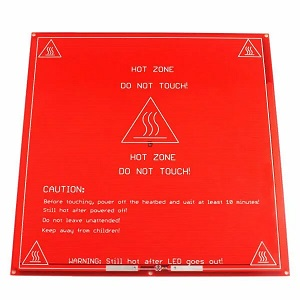
\includegraphics[width=8cm]{Heatbed}
\caption{\Large 加熱床(PCB heatbed)}\label{Heatbed}
\end{center}
\end{figure}
\begin{figure}[hbt!]
\begin{center}
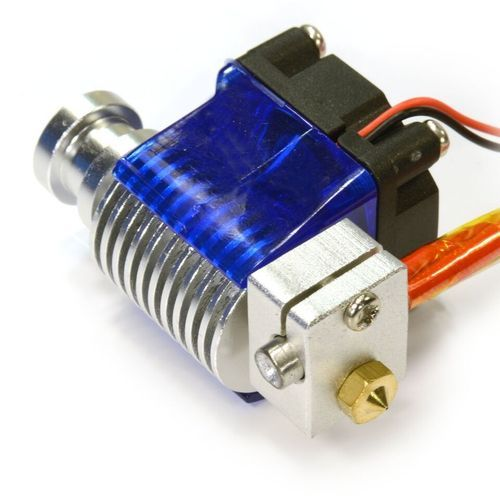
\includegraphics[width=8cm]{Extruder}
\caption{\Large 擠製頭(E3d V6 Hotend)}\label{Extruder}
\end{center}
\end{figure}
\begin{figure}[hbt!]
\begin{center}
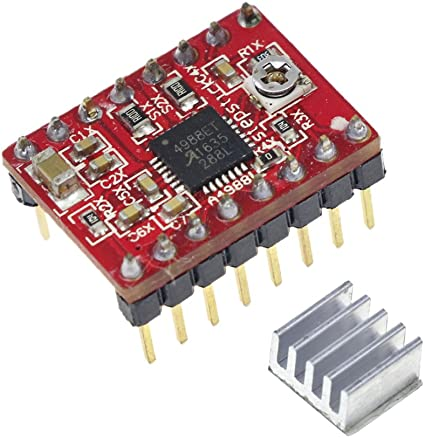
\includegraphics[width=8cm]{A4988}
\caption{\Large A4988 步進馬達驅動器(A4988 Stepper Motor Driver)}\label{A4988}
\end{center}
\end{figure}
\begin{figure}[hbt!]
\begin{center}
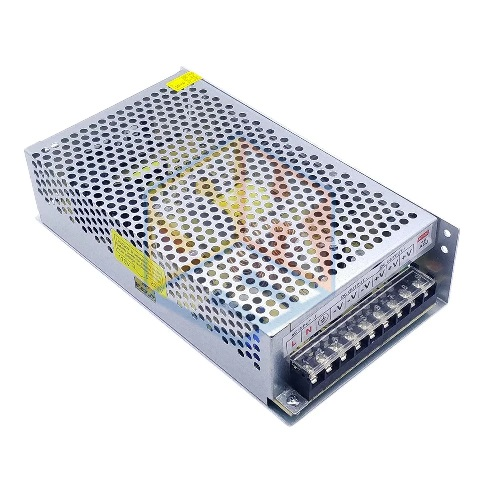
\includegraphics[width=8cm]{Power}
\caption{\Large 電源 12V/20A(Power supply 12V/20A)}\label{Power}
\end{center}
\end{figure}

\newpage 